% !TeX root = ../main.tex

\section{Background}

Hidden Markov models are useful when inferring a single unobserved process, but biological processes often involve multiple simultaneous hidden processes which can occur and at different time scales. For example, a preliminary observation of the killer whale dive data shown in figure (\ref{fig:data}) shows that the behavior of this killer whale changes between approximately hour-long periods of predominately short, shallow dives and long, deep dives. Leos-Barajas et al. encounter a similar issue when modeling the movement of a harbor porpoise in the North Sea, and use it as a motivating example when they introduce hierarchical hidden Markov models.

\begin{figure}[h!]
	\centering
	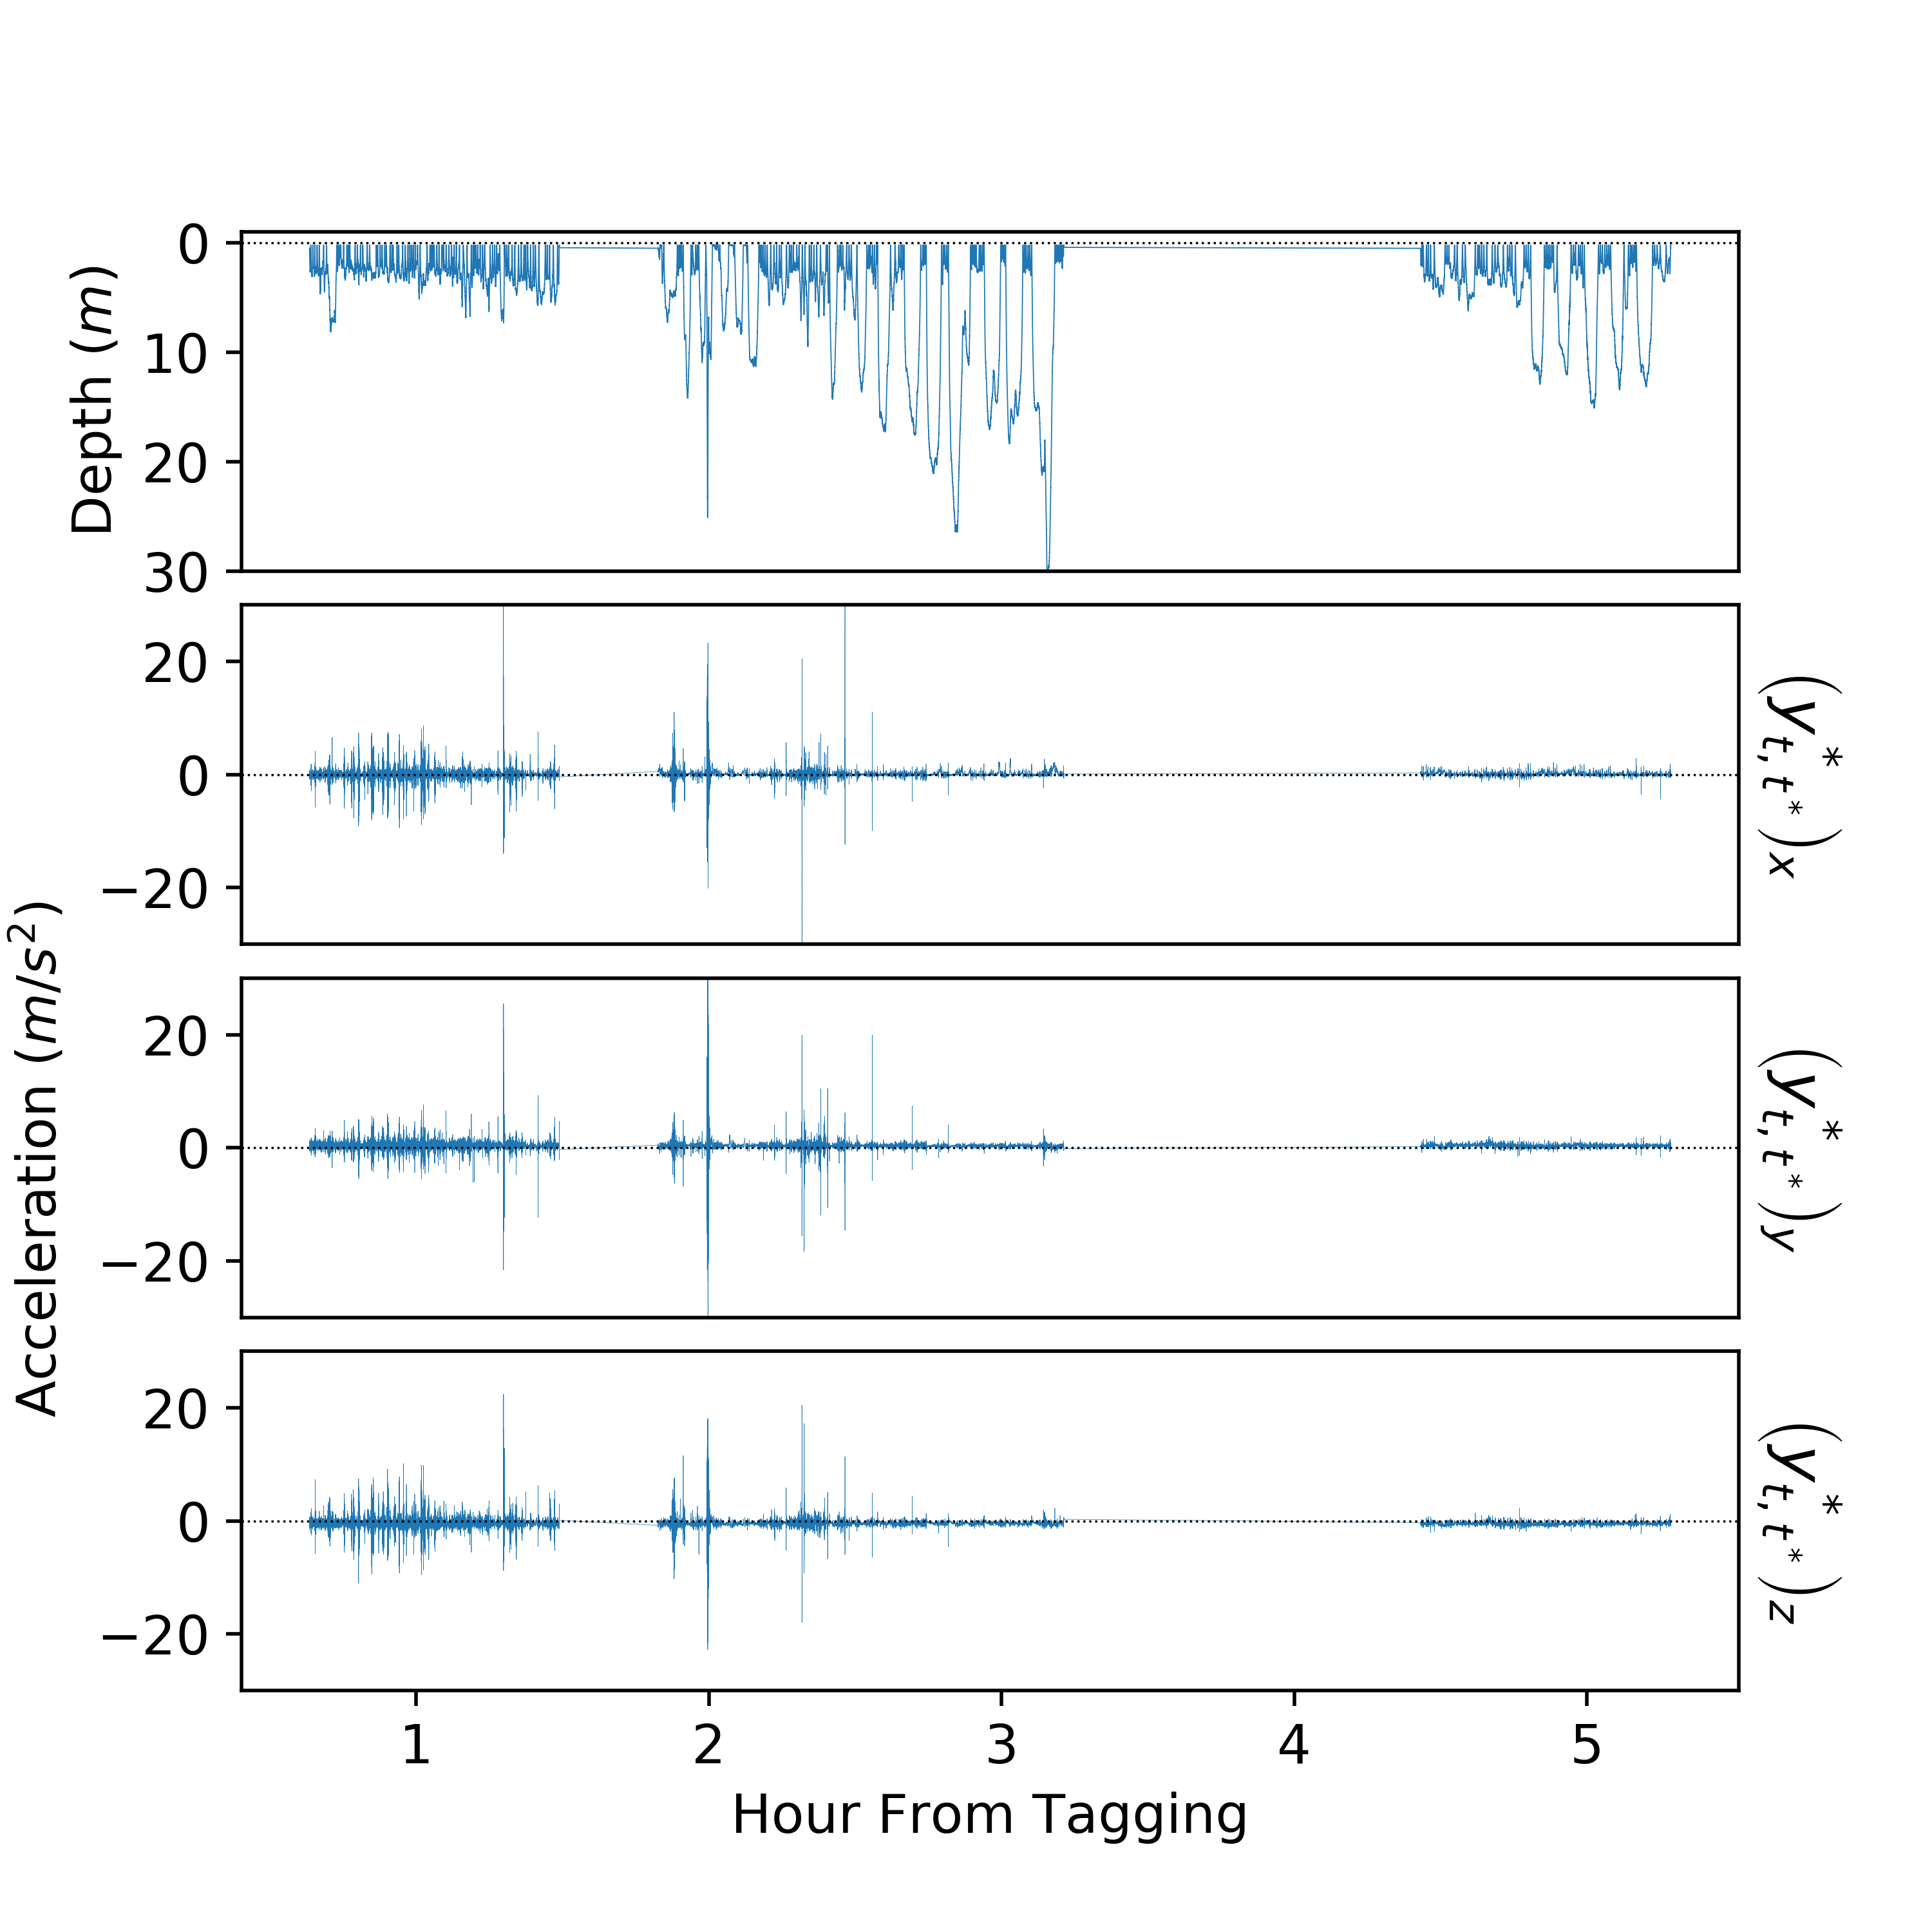
\includegraphics[width=6.5in]{../Plots/raw_data.png}
	\caption{Raw depth data of a Killer Whale off the coast of British Columbia, Canada.}
	\label{fig:data}
\end{figure}

\subsection{Hidden Markov models}
\label{subsection:HMMs}

\textit{Hidden Markov models} (or HMMs) are comprised of a sequence of unobserved states, $X_t$ $(t = 1, \ldots, T)$ which form a Markov chain and a sequence of (possibly high-dimensional) observations $Y_t$ $(t = 1, \ldots, T)$ which are often referred to as ``emissions". The index $t$ often represents equi-spaced jumps in time. In the field of animal movement, the unobserved chain usually represents the latent behaviour of an animal (e.g. foraging, resting, migrating, etc.), while the observations are often a series of step lengths and turning angles for land animals and either depth or accelerometer data (or both) for marine animals. Each random variable in the unobserved chain $X_t$ can take one of $N$ possible values, and $X$ has corresponding initial distribution $\delta \in \bbR^N$ and probability transition matrix $\Gamma \in \bbR^{N \times N}$:

$$\delta_i = Pr(X_1 = i); \quad i = 1,\ldots,N$$

$$\Gamma_{ij} = Pr(X_{t+1} = j | X_t = i); \quad t = 1, \ldots, T-1; \enspace i = 1,\ldots,N; \enspace j=1,\ldots,N $$

$\delta$ is often assumed to be the stationary distribution of the $\Gamma$- an assumption that we make in this work. Further, the distribution of each observation $Y_t$ depends only on the value of $X_t$ and none of the preceding observations or behavioral states, i.e. $p(y_t|x_1,\ldots, x_N, y_1,\ldots,y_{t-1},y_{t+1},\ldots,y_N) = p(y_t|x_t)$. In particular, we denote the distribution of $Y_t$ given $X_t = s$ as $f_s(y_t)$. $f_1,\ldots,f_N$ in turn depend upon a vector of parameters $\Theta = (\theta_1,\ldots,\theta_N)$ and hereafter are referred to as ``emission distributions". A visualization of the dependence structure can be seen in figure (\ref{fig:HMM}).
In order to estimate the parameters of an HMM, suppose data $y = (y_1,\ldots,y_T)$ is observed as a realization of an unknown HMM model. The probability transition matrix $\Gamma$, and parameters of the emission distributions $\Theta$ can be estimated by maximizing the likelihood of $y$, which we denote as $\calL_{\text{HMM}}(y;\Theta,\Gamma)$, with respect to $\Gamma$, $\delta$, and $\Theta$. In addition, $\calL_{\text{HMM}}(y;\theta,\Gamma,\delta)$ can be calculated using the \textit{forward algorithm} \cite{Zucchini:2016} as follows:
%
$$\calL_{\text{HMM}}(y;\theta,\Gamma) = \delta P(y_1;\theta) \prod_{t=2}^T \Gamma P(y_t;\theta) \mathbf{1}$$
%
where $\mathbf{1}_N$ is an $N$-dimensional column vector of ones, and:
%
$$P(y_t;\theta) = \text{diag}(f_1(y_t),\ldots , f_N(y_t)).$$
%
In order to ensure remove constraints when maximizing $\calL_{\text{HMM}}(y)$, $\Gamma$ is often parameterized using $\eta \in \bbR^{N \times N}$ and the following link function:
%
$$\Gamma_{ij} = \frac{\exp(\eta_{ij})}{\sum_{k=1}^N \exp(\eta_{ik})}, \qquad \eta_{ii} = 0 \quad \forall i \in \{1, \ldots, N\}.$$
%
$\eta_{ii}$ is set to zero for identifiability. $\calL_{\text{HMM}}(y;\theta,\Gamma)$ can be maximized using any numerical optimizer.

\begin{figure}[h!]
	\centering
	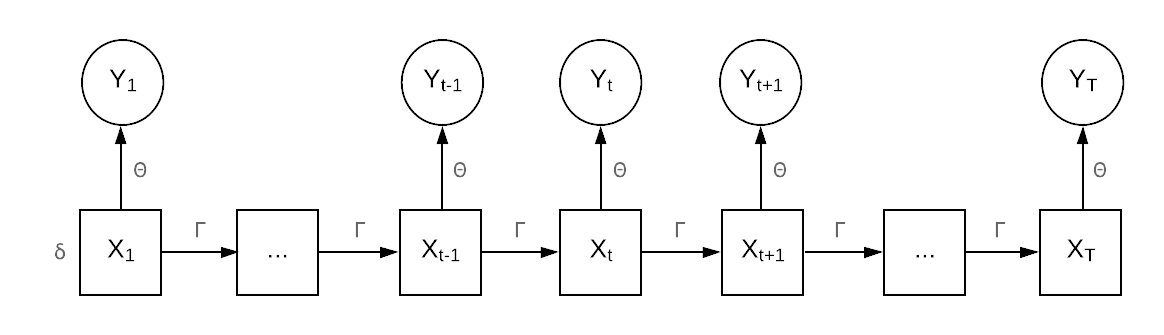
\includegraphics[width=5in]{../Plots/HMM.png}
	\caption{Graphical representation of a traditional HMM.}
	\label{fig:HMM}
\end{figure}


\subsection{Hierarchical HMMs}

A hierarchical hidden Markov model (or HHMM) is a variation of a hidden Markov model in which $X_t$ satisfies the conditions of section \ref{subsection:HMMs}, but in addition it produces yet another fine-scale hidden Markov model of length $T_t^*$. This fine-scale hidden Markov model can be either instead of \cite{Barajas:2017} or in addition to \cite{Adam:2019} a coarse-scale observation $Y_t$ which must satisfy the conditions of section \ref{subsection:HMMs}. The fine-scale HMM is comprised of a fine-scale Markov chain $X^*_t = (X^*_{t,1}, \ldots, X^*_{t,T^*_t})$ and fine-scale observations $Y^*_t = (Y^*_{t,1}, \ldots, Y^*_{t,T^*_t})$, each of length $T^*_t$. $X^*_t$ can take one of $N^*$ values. Note that while $N^*$ can be set to depend upon $X_t$, we assume here that it does not for simplicity in both the model and the notation. $X^*_t$ is characterized by an initial distribution $\delta^{*(X_t)} \in \bbR^{N^*}$ and probability transition matrix $\Gamma^{*(X_t)} \in \bbR^{N^* \times N^*}$:
%
$$\delta^{*(s)}_i = Pr(X^*_{t,1} = i | X_t = s); \quad i = 1,\ldots,N^*$$
%
$$\Gamma^{*(s)}_{ij} = Pr(X^*_{t,t^*+1} = j | X^*_{t,t^*} = i, X_t = s); \quad t^* = 1, \ldots, T^*_t-1; \enspace i,j = 1,\ldots,N^*$$
%
Again, we assume that the initial distribution $\delta^{*(s)}$ is the stationary distribution of $\Gamma^{*(s)}$. Each fine-scale observation $Y^*_{t,t^*}$ depends only on the value of its corresponding fine-scale hidden state $X^*_{t,t^*}$ and coarse-scale hidden state, $X_t$. We denote the distribution of $Y^*_{t,t^*}$ given that $X_t = s$ and $X^*_{t,t^*} = s^*$ as $f_{s,s^*}$. Therefore, in the hierarchical setting $\Theta$ is a $N$-by-$N^*$ matrix of parameters where $\theta_{s,s^*}$ describes the distribution $f_{s,s^*}$. Note the parameters of the fine-scale hidden Markov model ($\Gamma^{*(X_t)}$, $\delta^{*(X_t)}$, and $\theta^{*(X_t)}$) all depend upon the hidden state of the \textit{crude-scale} hidden Markov model. However, depending upon the discretion of the researcher, it is possible to force any of these parameters to be independent of the crude-scale hidden state $X_t$. A visualization of the full structure of the HHMM can be seen in figure (\ref{fig:HHMM}). Due to the nested structure of a hierarchical hidden Markov model, the likelihood of an HHMM is still easy to calculate using the forward algorithm:
%
$$\calL_{\text{HHMM}}(y,y^*;\theta,\theta^*,\Gamma,\Gamma^*,\delta,\delta^*) = \delta P(y_1,y_1^*;\theta,\theta^*,\Gamma^*,\delta^*) \prod_{t=2}^T \Gamma P(y_t,y_t^*;\theta,\theta^*,\Gamma^*,\delta^*) \mathbf{1}$$
%
where:
%
\begin{align*}
	P(y_t,y_t^*;\theta,\theta^*,\Gamma^*,\delta^*)  = \text{diag}\left[p_{\theta}(y_t|x_t = x_1)\calL_{\text{HMM}}\left(y_t^*;\theta^{*(x_1)},\Gamma^{*(x_1)},\delta^{*(x_1)}\right), . . . , \right.\\
	\left. p_{\theta}(y_t|x_t = x_N )\calL_{\text{HMM}}\left(y_t^*;\theta^{*(x_N)},\Gamma^{*(x_N)},\delta^{*(x_N)}\right) \right]
\end{align*}
%
Note that this formulation assumes that the crude-scale observations at a given time $Y_t$ and the fine-scale observation time series $Y_t^*$ are independent of one another when conditioned on $X_t$. For more information on specific considerations for HHMMs such as incorporating covariates into the probability transition matrix, model selection and model checking, see Adam et al \cite{Adam:2019}.

\begin{figure}[h!]
	\centering
	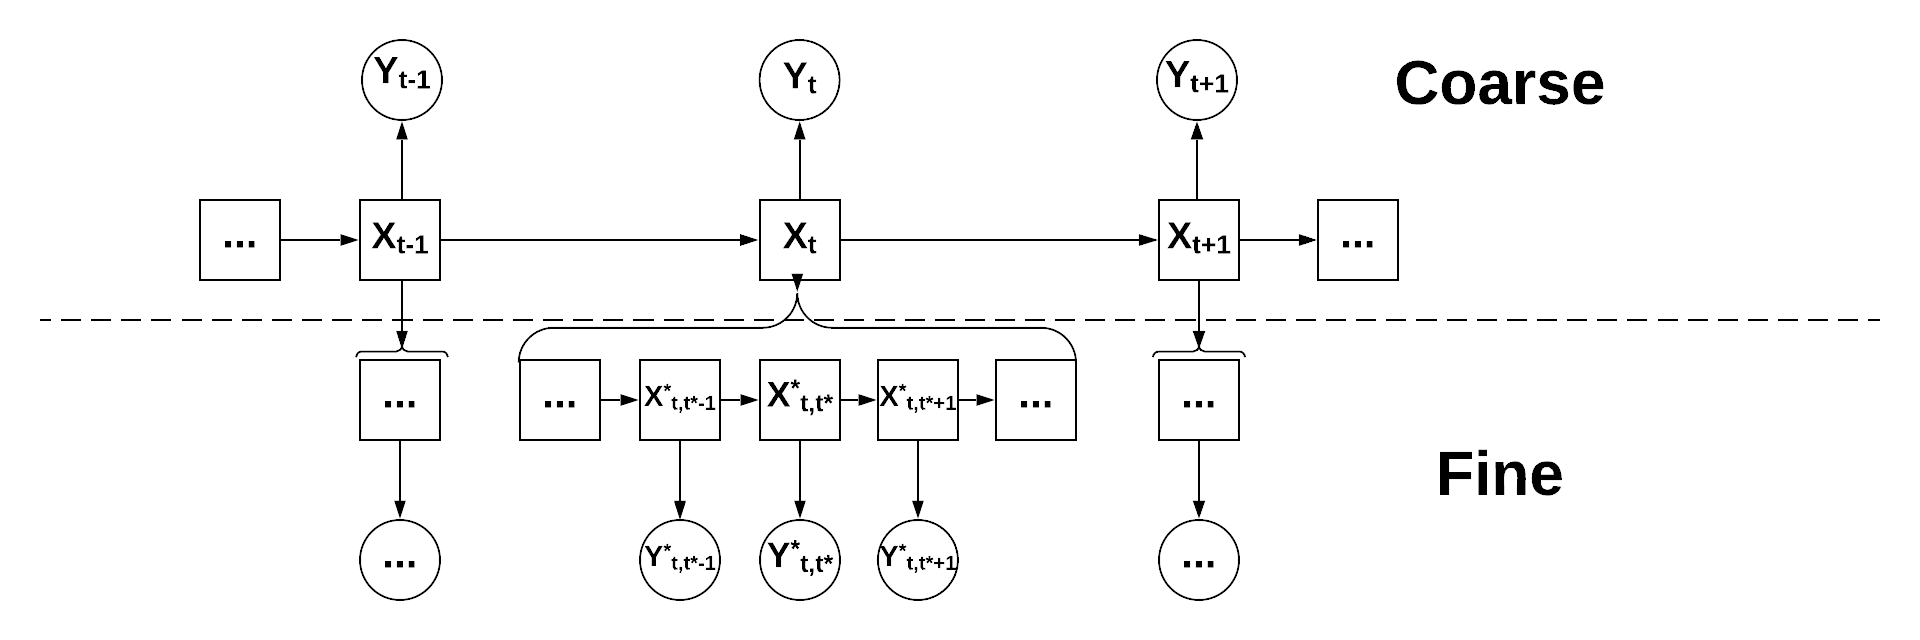
\includegraphics[width=6.5in]{../Plots/HHMM.png}
	\caption{Graphical representation of a traditional HHMM.}
	\label{fig:HHMM}
\end{figure}


\subsection{Conditionally auto-regressive HMMs}

One of the key assumptions of both HMMs and HHMMs is \textit{conditional Independence} between observations at both the crude and fine scale. Namely, given the state $X_t$ or $X^*_{t,t^*}$, $Y_t$ or $Y^*_{t,t^*}$ (respectively) is assumed to be independent from all other observations. Therefore, traditional HMMs and HHMMs can fail when the observation sequence $Y$ exhibits significant auto-correlation in time. Examples include fluking in marine mammals in Vancouver, BC (see the results section) and the swimming behavior of horn sharks off the coast of Southern California \cite{Adam:2019}.

One way to deal with auto-correlation in fine-scale behavioral processes is to use the CarHMM, or \textit{conditionally auto-regressive hidden Markov model}, introduced by Lawler et al \cite{Lawler:2019}. If the emission distribution of observation $Y_t$ is parameterized by its mean and variance, i.e. $\theta_{x_t} = \{\mu_{x_t},\sigma^2_{x_t}\}$, then the CarHMM models the distribution of $Y_t|X_t,Y_{t-1}$ as the following:
%
$$\mathbb{E}(Y_t) = \phi_{x_t}*Y_{t-1} + (1-\phi_{x_t}) * \mu_{x_t}$$
$$\mathbb{V}(Y_t) = \sigma^2_{x_t}$$
%
The CarHMM therefore explicitly models auto-correlation into the emission distributions of the HMM while maintaining the structure needed to run the forward algorithm and only adding one additional parameter per observation and hidden state. 

The likelihood of CarHMM is still compatible with the forward algorithm:
\begin{equation}
\calL_{\text{CarHMM}}(y) = \delta \prod_{t=2}^T \Gamma P(y_t;\theta) \mathbf{1}
\label{CarHMM_likelihood}
\end{equation}
where:
%
$$P(y_t;\theta) = \text{diag}(p_\theta(y_t|y_{t-1},X_t = x_1), . . . , p_\theta(y_t|y_{t-1},X_t = x_N )), \qquad t > 1$$
%
and the first observation $y_1$ is assumed to be fixed as an initial value. The graphical model associated with the structure of a CarHMM is shown in figure (\ref{fig:CarHMM}).

\begin{figure}[h!]
	\centering
	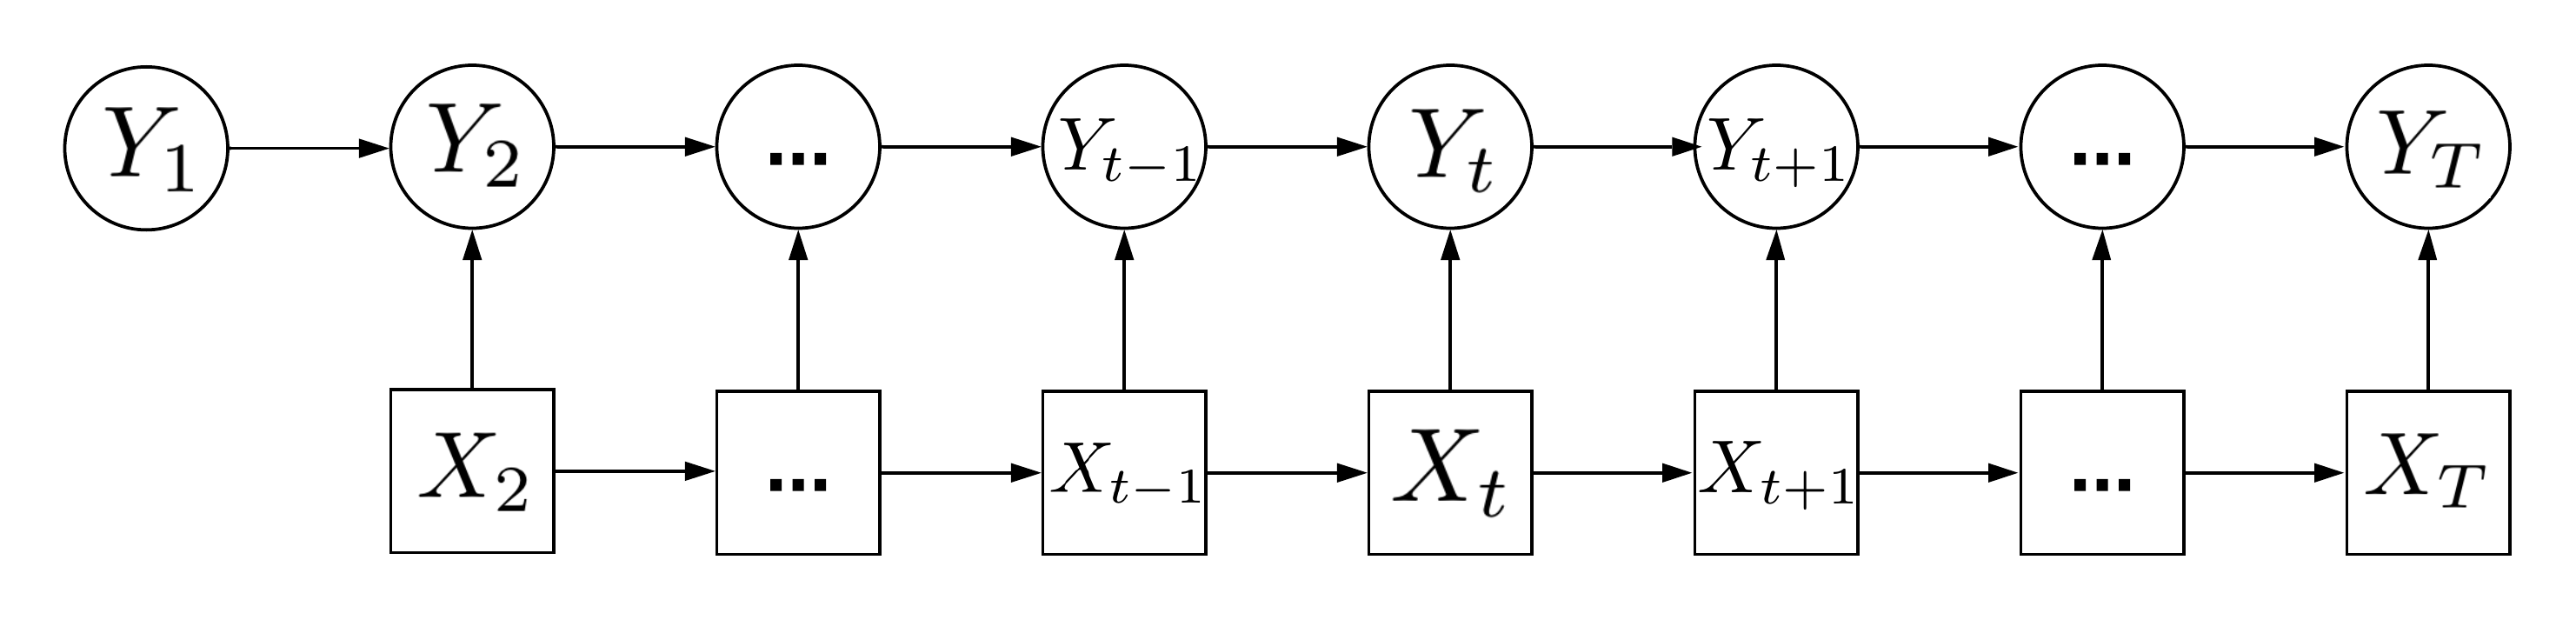
\includegraphics[width=3in]{../Plots/CarHMM.png}
	\caption{Graphical representation of a traditional CarHMM. The additional arrows representing auto-correlation between observations are shown in red for emphasis.}
	\label{fig:CarHMM}
\end{figure}


\subsection{State decoding}

Once an HMM, HHMM, or CarHMM model is fit by maximizing their respective likelihoods with respect to their parameters, it is common to find the most likely sequence of hidden states $\hat X$. 

This can be done in one of two ways: first, the \textit{most likely sequence} of \text{all} hidden states $\hat X$ is often found using a dynamic programming algorithm called the Viterbi algorithm \cite{Viterbi:1967}. Second, the \textit{probability} of \textit{each} crude-level state (conditioned on the learned parameters) can be found using the \textit{forward-backward algorithm}. In the case of HHMMs, both the Viterbi algorithm and the forward-backward algorithm are easy to extend to HHMMs by recursively running the algorithm on the fine-scale HMMs after decoding the states of the coarse-scale HMM.

While both the Viterbi algorithm and the forward-backward algorithm are used in the current ecology literature, we use the \textit{forward-backward algorithm} in this work for several reasons. In particular, the forward-backward algorithm is used to find the \textit{psuedoresiduals} of a given model, which is an important tool for model validation. In addition, for HHMMs the forward-backward algorithm can be used recursively to find the probability of the fine-level states $X^*_{t^*,t}$ exactly by marginalizing out $X_t$:
%
$$P(X^*_{t^*,t} = x^*_{t^*,t}) = \sum_{n=1}^N P(X_t = x_n)P(X^*_{t^*,t} = x^*_{t^*,t} | X_t = x_n)$$
%
where $P(X_t = x_n)$ can be found using the forward-backward algorithm on the crude-level Markov chain and $P(X^*_{s,t} = x^*_{s,t} | X_t = x_n)$ can be found by running the forward-backward algorithm on the fine-level HMM for every possible value of $X_t$.